\documentclass{standalone}
\usepackage{tikz}
\usetikzlibrary{patterns}
\usetikzlibrary{positioning}
\usetikzlibrary{patterns, positioning}
\usetikzlibrary{shapes.misc}
\usepackage[outline]{contour}
\contourlength{1.5pt} 
\usepackage[sfdefault]{ClearSans}

\begin{document}
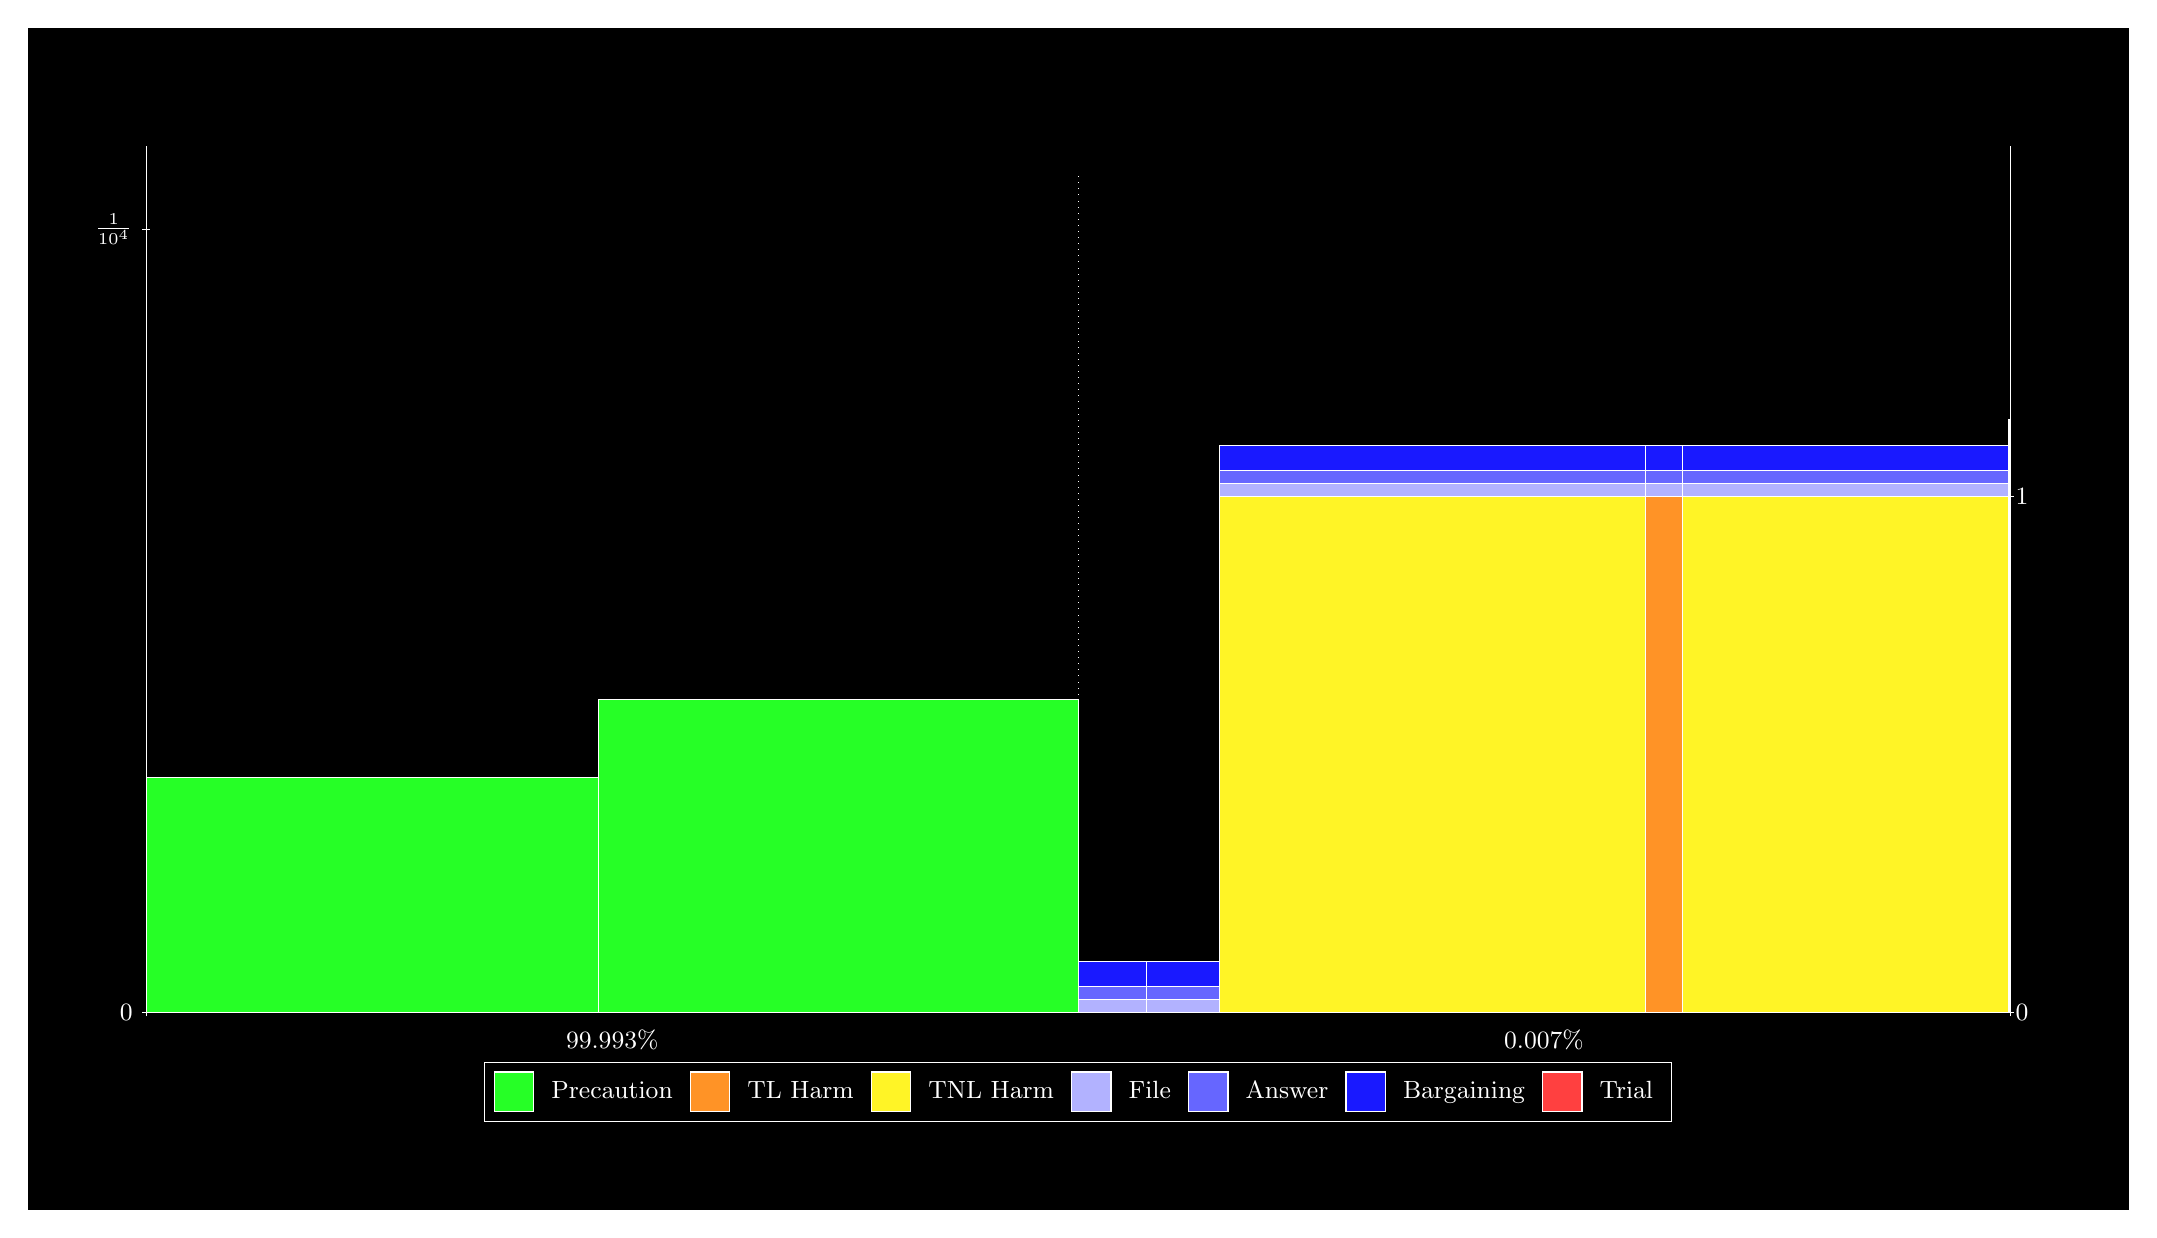
\begin{tikzpicture}
\draw[fill=black] (0,0) rectangle (26.667,15);
\draw[fill=green!85,draw=white,very thin] (1.5,2.5) rectangle (7.2428,5.4851);
\draw[fill=green!85,draw=white,very thin] (7.2428,2.5) rectangle (13.333,6.4801);
\draw[fill=green!85,draw=white,very thin] (13.333,2.5) rectangle (14.203,2.5002);
\draw[fill=blue!30,draw=white,very thin] (13.333,2.5002) rectangle (14.203,2.664);
\draw[fill=blue!60,draw=white,very thin] (13.333,2.664) rectangle (14.203,2.8278);
\draw[fill=blue!90,draw=white,very thin] (13.333,2.8278) rectangle (14.203,3.1554);
\draw[fill=green!85,draw=white,very thin] (14.203,2.5) rectangle (15.128,2.5003);
\draw[fill=blue!30,draw=white,very thin] (14.203,2.5003) rectangle (15.128,2.6641);
\draw[fill=blue!60,draw=white,very thin] (14.203,2.6641) rectangle (15.128,2.8279);
\draw[fill=blue!90,draw=white,very thin] (14.203,2.8279) rectangle (15.128,3.1555);
\draw[fill=green!85,draw=white,very thin] (15.128,2.5) rectangle (20.542,2.5002);
\draw[fill=yellow!85,draw=white,very thin] (15.128,2.5002) rectangle (20.542,9.0525);
\draw[fill=blue!30,draw=white,very thin] (15.128,9.0525) rectangle (20.542,9.2163);
\draw[fill=blue!60,draw=white,very thin] (15.128,9.2163) rectangle (20.542,9.3801);
\draw[fill=blue!90,draw=white,very thin] (15.128,9.3801) rectangle (20.542,9.7077);
\draw[fill=green!85,draw=white,very thin] (20.542,2.5) rectangle (21,2.5002);
\draw[fill=orange!85,draw=white,very thin] (20.542,2.5002) rectangle (21,9.0525);
\draw[fill=blue!30,draw=white,very thin] (20.542,9.0525) rectangle (21,9.2163);
\draw[fill=blue!60,draw=white,very thin] (20.542,9.2163) rectangle (21,9.3801);
\draw[fill=blue!90,draw=white,very thin] (20.542,9.3801) rectangle (21,9.7077);
\draw[fill=green!85,draw=white,very thin] (21,2.5) rectangle (25.151,2.5003);
\draw[fill=yellow!85,draw=white,very thin] (21,2.5003) rectangle (25.151,9.0526);
\draw[fill=blue!30,draw=white,very thin] (21,9.0526) rectangle (25.151,9.2164);
\draw[fill=blue!60,draw=white,very thin] (21,9.2164) rectangle (25.151,9.3802);
\draw[fill=blue!90,draw=white,very thin] (21,9.3802) rectangle (25.151,9.7078);
\draw[fill=green!85,draw=white,very thin] (25.151,2.5) rectangle (25.163,2.5002);
\draw[fill=yellow!85,draw=white,very thin] (25.151,2.5002) rectangle (25.163,9.0525);
\draw[fill=blue!30,draw=white,very thin] (25.151,9.0525) rectangle (25.163,9.2163);
\draw[fill=blue!60,draw=white,very thin] (25.151,9.2163) rectangle (25.163,9.3801);
\draw[fill=blue!90,draw=white,very thin] (25.151,9.3801) rectangle (25.163,9.7077);
\draw[fill=red!75,draw=white,very thin] (25.151,9.7077) rectangle (25.163,10.035);
\draw[fill=green!85,draw=white,very thin] (25.163,2.5) rectangle (25.167,2.5002);
\draw[fill=orange!85,draw=white,very thin] (25.163,2.5002) rectangle (25.167,9.0525);
\draw[fill=blue!30,draw=white,very thin] (25.163,9.0525) rectangle (25.167,9.2163);
\draw[fill=blue!60,draw=white,very thin] (25.163,9.2163) rectangle (25.167,9.3801);
\draw[fill=blue!90,draw=white,very thin] (25.163,9.3801) rectangle (25.167,9.7077);
\draw[fill=red!75,draw=white,very thin] (25.163,9.7077) rectangle (25.167,10.035);
\draw[white,very thin] (1.5,2.5) -- (1.5,13.5);
\draw[white,very thin] (1.45,2.5) -- (1.55,2.5);
\node[font=\small,text=white, anchor=east] at (1.45, 2.5) {0};
\draw[white,very thin] (1.45,12.45) -- (1.55,12.45);
\node[font=\small,text=white, anchor=east] at (1.45, 12.45) {$\frac{1}{10^{4}}$};

\draw[white,dotted,very thin] (13.333,2.83) -- (13.333,13.17);
\draw[white,very thin] (25.167,2.5) -- (25.167,13.5);
\draw[white,very thin] (25.117,2.5) -- (25.217,2.5);
\node[font=\small,text=white, anchor=west] at (25.117, 2.5) {0};
\draw[white,very thin] (25.117,9.0523) -- (25.217,9.0523);
\node[font=\small,text=white, anchor=west] at (25.117, 9.0523) {1};

\draw[white,very thin] (1.5,2.5) -- (25.167,2.5);
\draw[white,very thin] (1.5,2.45) -- (1.5,2.55);
\node[font=\small,text=white, anchor=north] at (1.5, 2.45) {};
\draw[white,very thin] (25.167,2.45) -- (25.167,2.55);
\node[font=\small,text=white, anchor=north] at (25.167, 2.45) {};

\node[font=\small,text=white,anchor=south] at (7.4167, 1.9) {99.993\%};
\node[font=\small,text=white,anchor=south] at (19.25, 1.9) {0.007\%};
\draw (13.3333,2.5) node (B) {};
\begin{scope}[align=center]
\matrix[scale=0.5,draw=white,below=0.5cm of B,nodes={draw},column sep=0.1cm]{
\node[rectangle,draw,minimum width=0.5cm,minimum height=0.5cm,fill=green!85]{}; & \node[draw=none,font=\small,text=white]{Precaution}; &
\node[rectangle,draw,minimum width=0.5cm,minimum height=0.5cm,fill=orange!85]{}; & \node[draw=none,font=\small,text=white]{TL Harm}; &
\node[rectangle,draw,minimum width=0.5cm,minimum height=0.5cm,fill=yellow!85]{}; & \node[draw=none,font=\small,text=white]{TNL Harm}; &
\node[rectangle,draw,minimum width=0.5cm,minimum height=0.5cm,fill=blue!30]{}; & \node[draw=none,font=\small,text=white]{File}; &
\node[rectangle,draw,minimum width=0.5cm,minimum height=0.5cm,fill=blue!60]{}; & \node[draw=none,font=\small,text=white]{Answer}; &
\node[rectangle,draw,minimum width=0.5cm,minimum height=0.5cm,fill=blue!90]{}; & \node[draw=none,font=\small,text=white]{Bargaining}; &
\node[rectangle,draw,minimum width=0.5cm,minimum height=0.5cm,fill=red!75]{}; & \node[draw=none,font=\small,text=white]{Trial}; \\\\
};\end{scope}

\end{tikzpicture}
\end{document}